\capitulo{3}{Conceptos teóricos}

%En aquellos proyectos que necesiten para su comprensión y desarrollo de unos conceptos teóricos de una determinada materia o de un determinado dominio de conocimiento, debe existir un apartado que sintetice dichos conceptos.
%
%Algunos conceptos teóricos de \LaTeX \footnote{Créditos a los proyectos de Álvaro López Cantero: Configurador de Presupuestos y Roberto Izquierdo Amo: PLQuiz}.
%
%\section{Secciones}
%
%Las secciones se incluyen con el comando section.
%
%\subsection{Subsecciones}
%
%Además de secciones tenemos subsecciones.
%
%\subsubsection{Subsubsecciones}
%
%Y subsecciones. 
%
%
%\section{Referencias}
%
%Las referencias se incluyen en el texto usando cite \cite{wiki:latex}. Para citar webs, artículos o libros \cite{koza92}.
%
%
%\section{Imágenes}
%
%Se pueden incluir imágenes con los comandos standard de \LaTeX, pero esta plantilla dispone de comandos propios como por ejemplo el siguiente:
%
%\imagen{escudoInfor}{Autómata para una expresión vacía}
%
%
%
%\section{Listas de items}
%
%Existen tres posibilidades:
%
%\begin{itemize}
%	\item primer item.
%	\item segundo item.
%\end{itemize}
%
%\begin{enumerate}
%	\item primer item.
%	\item segundo item.
%\end{enumerate}
%
%\begin{description}
%	\item[Primer item] más información sobre el primer item.
%	\item[Segundo item] más información sobre el segundo item.
%\end{description}
%	
%\begin{itemize}
%\item 
%\end{itemize}
%
%\section{Tablas}
%
%Igualmente se pueden usar los comandos específicos de \LaTeX o bien usar alguno de los comandos de la plantilla.
%
%\tablaSmall{Herramientas y tecnologías utilizadas en cada parte del proyecto}{l c c c c}{herramientasportipodeuso}
%{ \multicolumn{1}{l}{Herramientas} & App AngularJS & API REST & BD & Memoria \\}{ 
%HTML5 & X & & &\\
%CSS3 & X & & &\\
%BOOTSTRAP & X & & &\\
%JavaScript & X & & &\\
%AngularJS & X & & &\\
%Bower & X & & &\\
%PHP & & X & &\\
%Karma + Jasmine & X & & &\\
%Slim framework & & X & &\\
%Idiorm & & X & &\\
%Composer & & X & &\\
%JSON & X & X & &\\
%PhpStorm & X & X & &\\
%MySQL & & & X &\\
%PhpMyAdmin & & & X &\\
%Git + BitBucket & X & X & X & X\\
%Mik\TeX{} & & & & X\\
%\TeX{}Maker & & & & X\\
%Astah & & & & X\\
%Balsamiq Mockups & X & & &\\
%VersionOne & X & X & X & X\\
%}
En este capítulo se explican conceptos relevantes para la comprensión de este proyecto y su contexto.
\section{Calidad de proceso y producto software}
Todo proyecto de software tienen como objetivo desarrollar software de alta calidad, que cumpla con los requisitos acordados. Sin embargo, la calidad de un producto de software no tiene que ver solo con que se cumplan todos los requisitos funcionales, sino también otros requerimientos no funcionales que no se incluyen en la especificación como los de mantenimiento.

%Comentar fig 25.3 - Ppales factores de la calidad de protducto software p561
Sommerville enumera en \textit{Software Engineering} \cite{sommerville_ingenierisoftware_2002} los principales factores que afectan a la calidad del producto, como se puede observar en la figura \ref{fig:M3-FactoresCalidad}:
\begin{itemize}
	\tightlist
	\item Calidad del proceso
	\item Tecnología de desarrollo
	\item Calidad del personal
	\item Costo, tiempo y duración
\end{itemize}
\begin{figure}[!h]
	\centering
	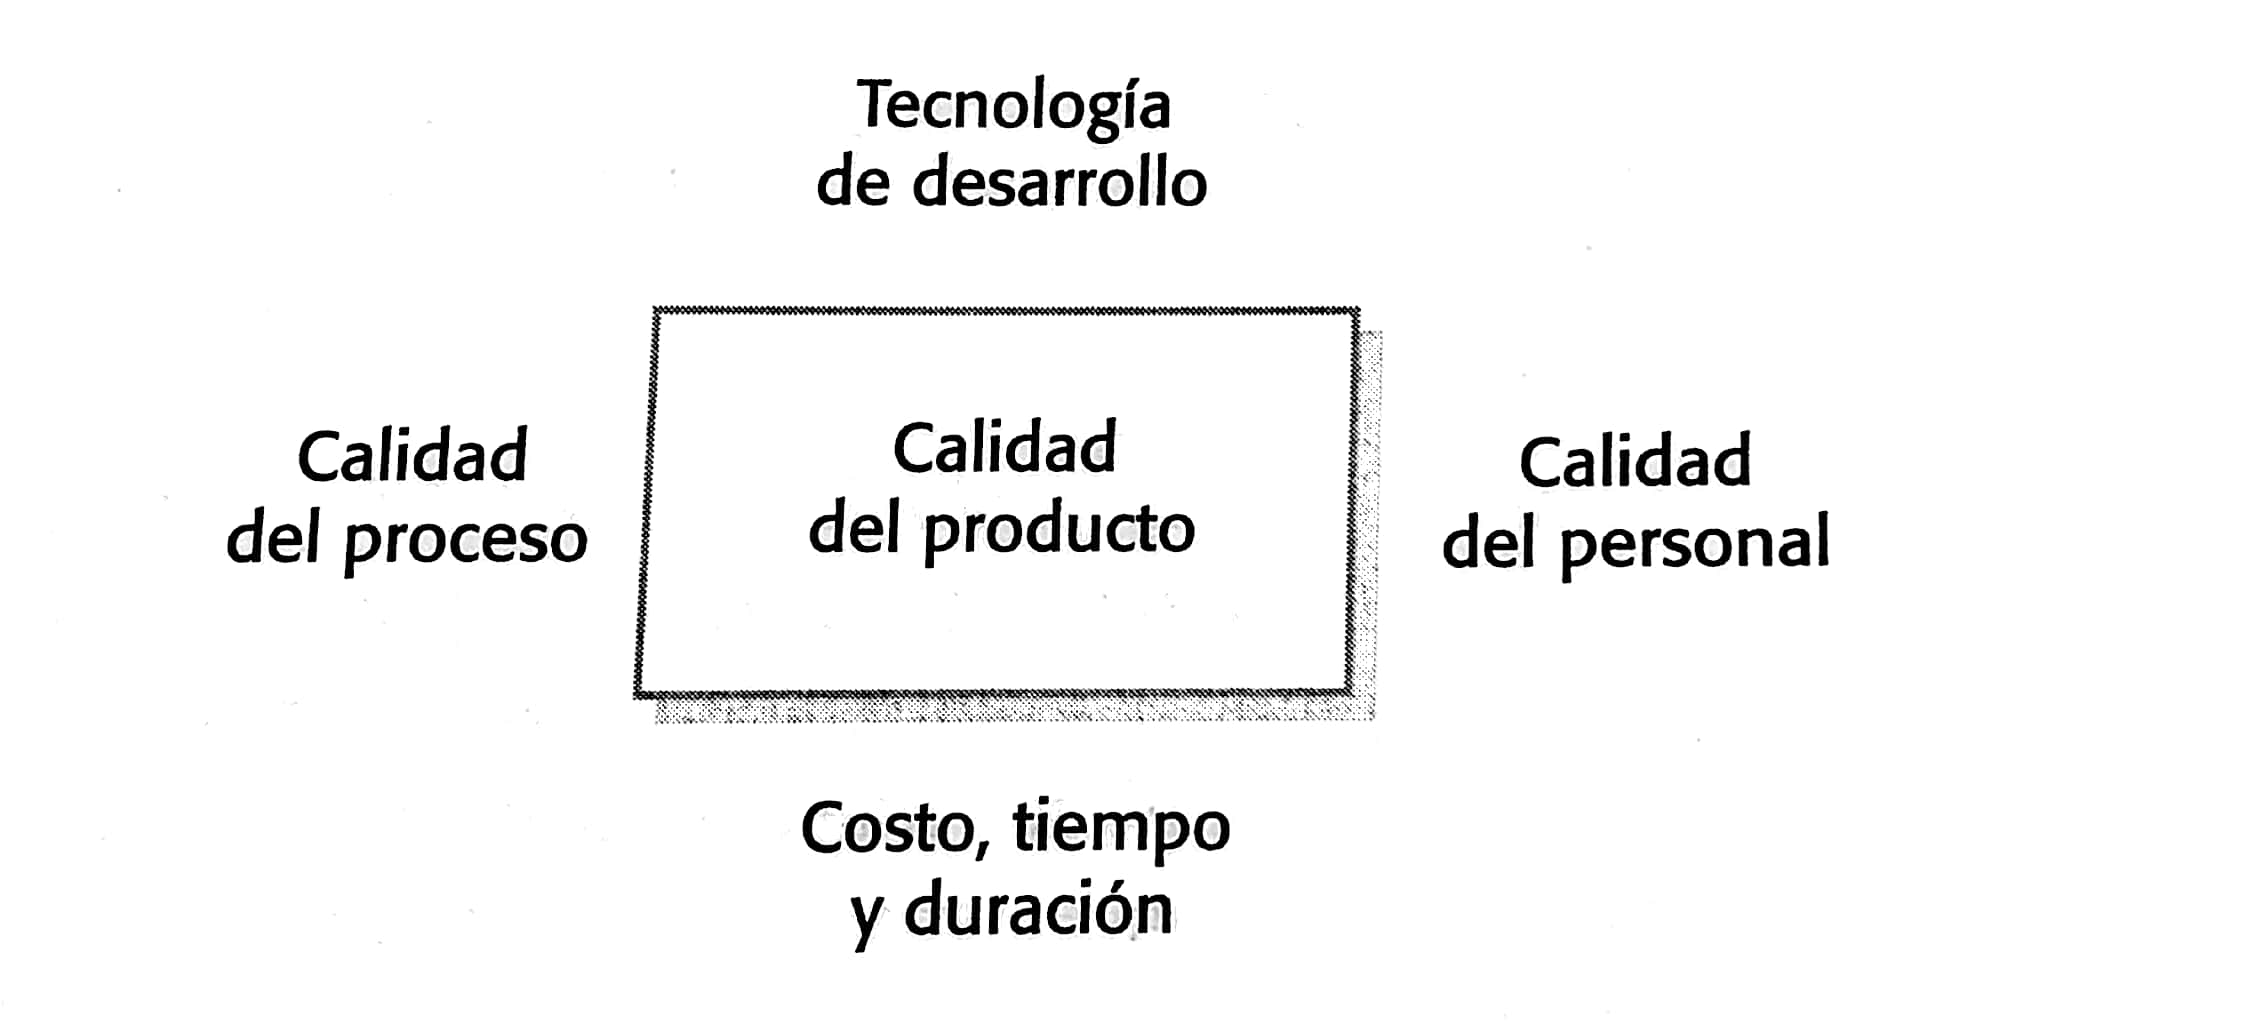
\includegraphics[scale=0.7]{M1-FactoresCalidad}
	\caption{Principales factores de calidad del producto de software\cite{sommerville_ingenierisoftware_2002}}\label{fig:M3-FactoresCalidad}
\end{figure}
\FloatBarrier

%Comentar fig 24.9 p549 relacion de metricas de proc y de prod

Para llegar a tener un software de calidad hay que tener en cuenta todos los factores mencionados anteriormente en cada una de las tres fases de la administración de la calidad: Aseguramiento, planeación y control.

La fase de control es la que se encarga de que el equipo de desarrollo cumpla los estándares y procedimientos definidos en el plan de calidad del proyecto. Esta fase puede realizarse mediante un proceso de medición.

La medición del software es un proceso en el cual se asignan valores numéricos o simbólicos a atributos de un producto o proceso software. Una métrica es una medida relacionada con un atributo de un proceso o producto software (por ejemplo). Las métricas son de control o de predicción. Las \textbf{métricas de control} se asocian al proceso de desarrollo del software (p. ej. Media de días ue se tarda en cerrar una incidencia )y las \textbf{métricas de predicción} se asocian a productos software (p. ej. Complejidad ciclomática de una función). Y ambos tipos de métricas influyen en la toma de decisiones administrativas como se observa en la figura \ref{fig:M3-MetricasProcesoYProducto}.
\begin{figure}[!h]
	\centering
	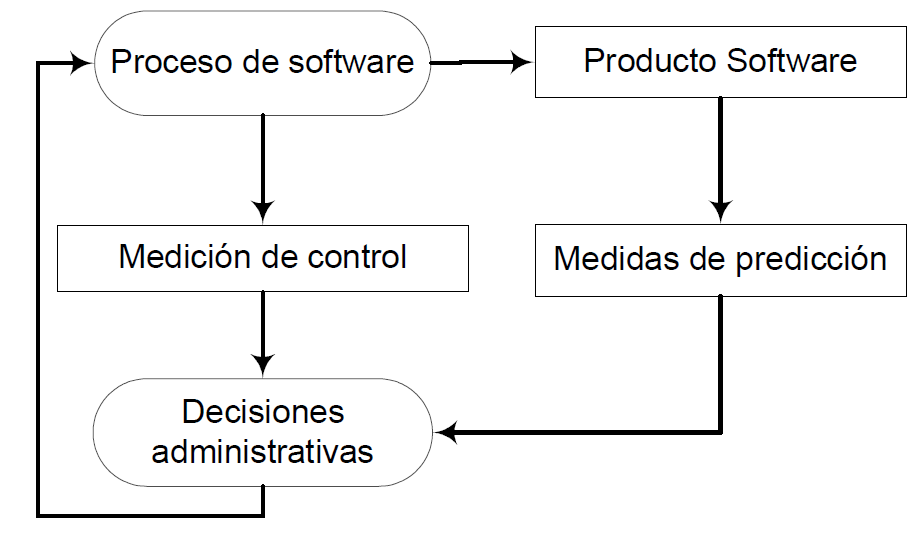
\includegraphics[scale=0.5]{M3-MetricasProcesoYProducto}
	\caption{Métricas de control y métricas de predicción\cite{sommerville_ingenierisoftware_2002}}\label{fig:M3-MetricasProcesoYProducto}
\end{figure}
%Comentar fg 24.1 p537 admin de calida en el proceso y desarrollo de software
\section{Evolución de software}
Este proyecto se centra en las métricas de control, es decir las que están asociadas al proceso de desarrollo o de evolución del software.
\subsection{Conceptos de evolución}
Un sistema de Gestión de Configuración del Software (SCM) es capaz de gestionar la evolución y cambios del código fuente en el tiempo \cite{berczuk_software_2002, sommerville_software_2016}.
En este apartado describiremos los conceptos básicos que utilizaremos para recoger, documentar, almacenar y recuperar los diferentes cambios que se produzcan en las entidades que formen parte nuestro sistema.
Un proyecto software está compuesto por múltiples ficheros y directorios. Llamaremos ítem a cualquier fichero o directorio cuya evolución en el tiempo está controlada por un sistema de Gestión de Configuración del Software (SCM). Una vez que estén bajo control, será posible ver su historial de cambios o revisiones y recuperar un estado anterior.
A medida que los ítems evolucionan en el tiempo, se van creando nuevas revisiones de los mismos. Como es lógico, algunos ítems sufrirán más cambios que otros a lo largo del desarrollo. El SCM almacena todas las revisiones de cada ítem, de manera que es posible volver al estado de uno de estos elementos en un momento dado.
La creación de revisiones ocurre a través de las operaciones de desprotección (check-out) y protección (check-in). Cuando se va a hacer una modificación en un ítem, éste se desprotege para editarlo. Para crear una nueva revisión del ítem de forma que se pueda recuperar su estado en este punto, se protege, lo que indica al SCM que debe almacenar los nuevos contenidos del ítem.
Al conjunto de revisiones de un ítem se le denomina historia y resume la evolución de ese ítem en el tiempo.
Una rama es un contenedor de revisiones, capaz de almacenar la evolución de los ítems como se muestra en la Ilustración 1. Las ramas pueden contener revisiones de más de un ítem. De hecho, esta es la situación más habitual.
Ilustración 1: Concepto de rama

Una etiqueta o label es el modo de marcar revisiones para poder agruparlas según un cierto criterio, que normalmente fija el usuario. Cuando se aplica una etiqueta, se crea una instantánea de la situación de los ítems en el tiempo. Más tarde esa instantánea puede ser referenciada con facilidad para identificar ese momento específico. Una etiqueta es, en definitiva, un nombre más fácil de recordar que se asigna a un conjunto particular de revisiones.
Las etiquetas se aplican siempre a las revisiones de los ítems que se encuentren actualmente en el espacio de trabajo o workspace, que es la zona donde el SCM puede mantener ítems bajo el control de versiones. A efectos prácticos, el workspace no dejará de ser un directorio en el disco.
Los ítems, sus revisiones, las ramas donde se almacenan las revisiones y las etiquetas que agrupan las revisiones se almacenan en un repositorio, que será el espacio principal donde el SCM guarda todos los objetos.


\subsection{Métricas de evolución}
Las métricas que se calculan de los proyectos son un conjunto de métricas que proceden de la Master Tesis titulada \textit{sPACE: Software Project Assessment in the Course of Evolution} \cite{ratzinger_space:_2007}.\\\\
\textbf{\underline{I1 - Número total de issues}}
\begin{itemize}
	\tightlist
	\item \textbf{Categoría}: Proceso de Orientación
	\item \textbf{Descripción}: Número total de issues creadas en el repositorio
	\item \textbf{Propósito}: ¿Cuántas issues se han definido en el repositorio?
	\item \textbf{Fórmula}: NTI. NTI = número total de issues
	\item \textbf{Fuente de medición}: Repositorio de un gestor de repositorios
	\item \textbf{Interpretación}: NTI >= 0. Valores bajos indican que no se utiliza un Sistema de seguimiento de incidencias, podría ser porque el proyecto acaba de comenzar
	\item \textbf{Tipo de escala}: Absoluta
	\item \textbf{Tipo de medida}: NTI = Contador
\end{itemize}
\textbf{\underline{I2 - Commits por issue}}
\begin{itemize}
	\tightlist
	\item \textbf{Categoría}: Proceso de Orientación
	\item \textbf{Descripción}: Número de commits por issue
	\item \textbf{Propósito}: ¿Cuántos commits realizados por cada issue?
	\item \textbf{Fórmula}: CI = NTC/NTI. NTI = Numero total de issues, NTC = Número total de commits
	\item \textbf{Fuente de medición}: Repositorio de un gestor de repositorios
	\item \textbf{Interpretación}: CI >= 0, Si se acerca a 1 se definen bien las issues, si alto: no se definen bien las issues, si bajo: desarrollo del proyecto lento
	\item \textbf{Tipo de escala}: Ratio 
	\item \textbf{Tipo de medida}: NTI, NTC = Contador
\end{itemize}
\textbf{\underline{I3 - Porcentaje de issues cerradas}}
\begin{itemize}
	\tightlist
	\item \textbf{Categoría}: Proceso de Orientación
	\item \textbf{Descripción}: Porcentaje de issues cerradas
	\item \textbf{Propósito}: ¿Qué porcentaje de issues definidas en el repositorio se han cerrado?
	\item \textbf{Fórmula}: PIC = NTIC*100/NTI. NTIC = Número total de issues cerradas, NTI = Numero total de issues
	\item \textbf{Fuente de medición}: Repositorio de un gestor de repositorios
	\item \textbf{Interpretación}: 0 <= PIC <= 100. Cuanto más alto mejor
	\item \textbf{Tipo de escala}: Ratio
	\item \textbf{Tipo de medida}: NTI, NTIC = Contador
\end{itemize}
\textbf{\underline{TI1 - Media de días en cerrar una issue}}
\begin{itemize}
	\tightlist
	\item \textbf{Categoría}: Constantes de tiempo
	\item \textbf{Descripción}:  Media de días en cerrar una issue
	\item \textbf{Propósito}: ¿Cuánto se suele tardar en cerrar una issue? 
	\item \textbf{Fórmula}: MDCI = SUM(DCI) / NTIC . NTIC = Número total de issues cerradas, DCI = Días en cerrar la issue
	\item \textbf{Fuente de medición}: Repositorio de un gestor de repositorios
	\item \textbf{Interpretación}: MDCI >= 0. Cuanto más pequeño mejor.
	\item \textbf{Tipo de escala}: Ratio
	\item \textbf{Tipo de medida}: NTI, NTIC = Contador
\end{itemize}
\textbf{\underline{TC1 - Media de días entre commits}}
\begin{itemize}
	\tightlist
	\item \textbf{Categoría}: Constantes de tiempo
	\item \textbf{Descripción}: Media de días que pasan entre dos commits consecutivos
	\item \textbf{Propósito}: ¿Cúanto tiempo suele pasar desde un commit hasta el siguiente?
	\item \textbf{Fórmula}: MDEC = [Sumatorio de (TCi-TCj) desde i=1, j=0 hasta i=NTC] / NTC. NTC = Número total de commits, TC = Tiempo de Commit 
	\item \textbf{Fuente de medición}: Repositorio de un gestor de repositorios
	\item \textbf{Interpretación}: MDEC >= 0. Cuanto más pequeño mejor.
	\item \textbf{Tipo de escala}: Ratio
	\item \textbf{Tipo de medida}: NTC = Contador; TC = Tiempo
\end{itemize}
\textbf{\underline{TC2 - Días entre primer y último commit}}
\begin{itemize}
	\tightlist
	\item \textbf{Categoría}: Constantes de tiempo
	\item \textbf{Descripción}: Días transcurridos entre el primer y el ultimo commit 
	\item \textbf{Propósito}: ¿Cuantos días han pasado entre el primer y el último commit?
	\item \textbf{Fórmula}: DEPUC = TC2- TC1. TC2 = Tiempo de último commit, TC1 = Tiempo de primer commit.
	\item \textbf{Fuente de medición}: Repositorio de un gestor de repositorios
	\item \textbf{Interpretación}: DEPUC >= 0
	\item \textbf{Tipo de escala}: Absoluta
	\item \textbf{Tipo de medida}: TC = Tiempo
\end{itemize}
\textbf{\underline{TC3 - Ratio de actividad de commits por mes}}
\begin{itemize}
	\tightlist
	\item \textbf{Categoría}: Constantes de tiempo
	\item \textbf{Descripción}: Muestra el número de commits relativos al número de meses
	\item \textbf{Propósito}:¿Cuál es el número medio de cambios por mes?
	\item \textbf{Fórmula}: RCM = NTC / 12
	\item \textbf{Fuente de medición}: Repositorio de un gestor de repositorios
	\item \textbf{Interpretación}: RCM > 0. Cuanto más alto mejor
	\item \textbf{Tipo de escala}: Ratio
	\item \textbf{Tipo de medida}: NTC = Contador
\end{itemize}
\textbf{\underline{C1 - Número de commits en el mes pico}}
\begin{itemize}
	\tightlist
	\item \textbf{Categoría}: Constantes de tiempo
	\item \textbf{Descripción}: Número de commits en el mes que más commits se han realizado en relación con el número total de commits
	\item \textbf{Propósito}: ¿Cuál es la proporción de trabajo realizado en el mes con mayor número de cambios?
	\item \textbf{Fórmula}: CCP = NCMP / NTC. NCMP = Número de commits en el mes pico, NTC = Número total de commits
	\item \textbf{Fuente de medición}: Repositorio de un gestor de repositorios
	\item \textbf{Interpretación}: 0 <= CCP <= 1. Mejor valores intermedios
	\item \textbf{Tipo de escala}: Ratio
	\item \textbf{Tipo de medida}: NCMP, NTC = Contador
\end{itemize}

\section{Framework de medición}
Para la implementación de las métricas se ha seguido la solución basada en frameworks propuesta en Soporte de Métricas con Independencia del Lenguaje para la Inferencia de Refactorizaciones [8]. Este framework (\ref{fig:MCTMotorMetricas}) es independiente del lenguaje y su objetivo es la reutilización en la implementación del cálculo de métricas.
%Describir el diseño del motor de métricas, nombrar puntos de extensión
\imagen{MCTMotorMetricas}{Diagrama del Framework para el cálculo de métricas con perfiles.}
